\section{September 7, 2023}

\subsection{Syllabus}

Prerequisites: 

\begin{itemize}
    \item know probability, random variables, expectation, distribution function, etc. don't need to know about measure theory. 
    \item calculus and lin alg. vectors, matrices, eigenvectors, eigenvalues  
\end{itemize}

\noindent Grading: 

\begin{itemize}
    \item 6 problem sets (40\%). lowest pset is dropped. since the lowest pset is dropped, late homework won't be accepted
    \item 2 midterms (60\%)
\end{itemize}

\subsection{General Outline}

Stochastic Processes are a family of random variables indexed by time. Rough outline of things that we'll cover in this class: 
\begin{enumerate}
    \item Markov Chain fundamentals 
    \item Countable state space markov chains (MC)
    \item Martingales, models of fair betting systems
    \item Continuous time/space MC
\end{enumerate}

\subsection{Intro}

Assume everything is discrete time for now. 

\begin{definition}
\deflabel

A \ac{stochastic process} is a sequence of r.v.s $X_1, X_1, \hdots$ jointly defined. 
\end{definition}

Think of the indices $1,2,\hdots$ as time. 

\begin{definition}
\deflabel

A \ac{Markov Chain} is a stochastic process $\{X_i\}$ taking values in $\mathcal{X}$ s.t. 
\[\PP[X_i=z_i | X_0=z_0,\hdots, X_{i-1} = z_{i-1}] = \PP[X_i=z_i | X_{i-1} = z_{i-1}].\] 
We call $\mathcal{X}$ the \ac{state space}. 
\end{definition}

Intuitively, the probability of any given state only relies on each state at the directly previous timestep. This is called the \ac{Markov property}. 

\begin{definition}
\deflabel

We say $X_i$ is \ac{time homogenous} if $\PP[X_i = z_i | X_{i-1} = z_{i-1}]$ is independent of $i$. 
\end{definition}

\noindent \textbf{In this course, we assume that all markov chains are time homogenous.}

\noindent Here are some common examples of Markov Chains: 

\begin{example}
\exlabelname{Gambler's Ruin}

Let $\mathcal{X} = \NN$, and $X_i$ be the amount of money a gambler has at time $i$, if they bet $\$1$ during each timestep. 
\end{example}

For example, if $X_0 = \$5$, then a valid sequence could be $5,6,7,6,5,4,\hdots$. 

\begin{example}
\exlabelname{Random Walk}

Let $G=(V,E)$. We move to a neighbor uniformly at random. 
\end{example}

\begin{definition}
\deflabel

Let $P^i(x,y) = \PP[X_i=y|X_0=x]$. 
\end{definition}

This is the probability of moving from $x$ to $y$ in $i$-steps starting from any point in time. The collection of probabilities $P^1(x,y) = P(x,y)$ is called the \ac{transition probabilities}. 

\begin{theorem}
\lemlabel

$P^i(x,y)$ is equal to the $(x,y)$th entry of $P^i$, where $P$ is a matrix of the transition probabilities. 
\end{theorem}

\begin{proof}
Proceed by induction on $i\geq 1$.

Base case $i=1$ is clear. 

Now, using inductive hypothesis and markov property, 
\begin{align*}
    \PP[X_{i+1}=y|X_0=x] &= \sum_z\PP[X_{i+1}=y|X_0=x, X_i=z]\cdot \PP[X_i=z|X_0=x] \\
    &= \sum_z P(z,y)P^i(x,z) = P^{i+1}(x,y).
\end{align*}
\end{proof}

\begin{theorem}
\lemlabel

Let $P$ be a markov chain and $\mu$ be a distribution on $\mathcal{X}$, viewed as a row vector. Then 
\[(\mu P^i)_x = \PP[X_i=x|X_0\sim \mu]. \]
\end{theorem}

The notation $X_0\sim \mu$ means that the initial state of the Markov chain is randomly drawn from $\mu$. 

\subsection{Visual Representation}

Draw a directed graph $G=(\mathcal{X}, E)$ where $(x,y)\in E$ if $P(x,y) > 0$, and label $(x,y)$ with $P(x,y)$.

\begin{example}
\exlabelname{Gambler's ruin}

\begin{center}
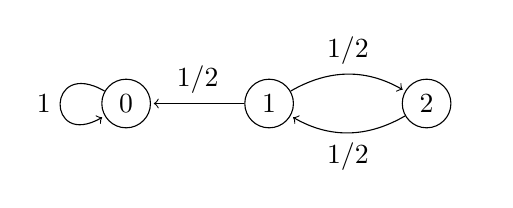
\begin{tikzpicture}[->, shorten >=1pt, scale=1, transform shape, node distance = 2cm]
    \node [circle, draw] (zero) {0};
    \node [circle, draw] (one) [right of=zero, right=-0.5cm] {1};
    \node [circle, draw] (two) [right of=one] {2};
    \node [] (three) [right of=two, right=-1.5cm] {$\hdots$};
    \path (zero) edge [loop left, in=210, out=150, looseness=7] node [left] {$1$} (zero);
    \path (one) edge [left] node [above] {$1/2$} (zero);
    \path (one) edge [bend left] node [above] {$1/2$} (two);
    \path (two) edge [bend left] node [below] {$1/2$} (one);
\end{tikzpicture}
\end{center}
\end{example}

\subsection{More definitions}

First goal: understand long-term behavior of markov chains. 

\begin{definition}
\deflabel

Let $P$ be a MC on $\mathcal{X}$. We say $x$ and $y$ \ac{communicate} and write $x\sim y$ if $\exists i,j > 0$ s.t. $P^i(x,y) > 0$ and $P^j(y,x) > 0$, or $x=y$. 
\end{definition}

\begin{theorem}
\lemlabelname{$\sim$ is an equivalence relation}

\begin{enumerate}
    \item $x\sim x$
    \item $x\sim y\implies y\sim x$
    \item $x\sim y, y\sim z\implies x\sim z$
\end{enumerate}
\end{theorem}

This implies a partition $\mathcal{X} = \mathcal{X}_1\cup \hdots \cup \mathcal{X}_k$, where $x\sim y$ iff $x,y\in \mathcal{X}_i$ for some $i$. 

\begin{definition}
\deflabel

We call these $\mathcal{X}_i$ \ac{communicating classes}. Moreover, we say a class $A$ is \ac{closed} if $P(x,y) = 0\forall x\in A, y\notin A$. 
\end{definition}

\begin{definition}
\deflabel

We say a markov chain is \ac{irreducible} if it has exactly one closed class. 
\end{definition}

\begin{theorem}
\proplabel

Every finite markov chain has a closed class. 
\end{theorem}

\begin{proof}
Let $A$,$B$ be communicating classes. Write $A\rightarrow B$ if $\exists x\in A, y\in B$ s.t. $P(x,y) > 0$. 

If $A\rightarrow B$, and $A\neq B$, then $B\not\rightarrow A$. Suppose there were no closed class. Then $\exists$ sequence $A_1\neq A_2\neq \hdots$ s.t. $A_1\rightarrow A_2\rightarrow \hdots$, since we can keep picking elements outside of non-closed classes. Given a finite number of elements, there is some $i,j$ such that $A_i=A_j$, contradiction.   
\end{proof}

Idea: closed classes are like irreducible Markov Chains. 